% main.tex
%=============================================================================
% Main document, including the IEEEtran preamble and content in one file

% Include the shared preamble
% Document class
\documentclass[conference,a4paper]{IEEEtran}

% Encoding and font
\usepackage[T1]{fontenc}
\usepackage[utf8]{inputenc}
\usepackage{lmodern}

% Graphics and paths
\usepackage{graphicx}
\graphicspath{{assets/images/}}
\usepackage{subcaption}

% Math packages
\usepackage{amsmath,amssymb}

% Hyperlinks
\usepackage[colorlinks=true, linkcolor=blue, urlcolor=blue, citecolor=blue]{hyperref}

% Color (for figures and highlights)
\usepackage{xcolor}

% Custom commands
% Example: Real numbers symbol
\newcommand{\R}{\mathbb{R}}

% Theorem environments (if needed)
\usepackage{amsthm}
\newtheorem{theorem}{Theorem}[section]
\newtheorem{lemma}[theorem]{Lemma}

\setlength{\marginparwidth}{2cm}
\usepackage{todonotes}
\usepackage{enumitem}
\usepackage{fancyhdr}

% Page layout adjustments (optional)
% \usepackage[margin=0.75in]{geometry}

% PDF metadata setup
\hypersetup{
  pdftitle    = {autowerkstatt4null: An Off-Board-Diagnostics Ecosystem for Car-Workshops},
  pdfauthor   = {Stephan Bökelmann, René Glitza, Gereon Kortenbruck, Lukas Jakubczyk, Meihui Huang, Odin Holmes},
  pdfsubject  = {Overview Paper for autowerkstatt4null},
  pdfkeywords = {AI diagnostics, federated learning, automotive workshops, oscilloscopes, GAIA-X, REST, WebSockets}
}


\begin{document}

% Title and Authors
\title{autowerkstatt4null: An Off-Board-Diagnostics Ecosystem for Car-Workshops}
\author{%
  \IEEEauthorblockN{%
    Stephan Bökelmann\IEEEauthorrefmark{1}, René Glitza\IEEEauthorrefmark{1},%
    Gereon Kortenbruck\IEEEauthorrefmark{2}, Lukas Jakubczyk\IEEEauthorrefmark{2},%
    Meihui Huang\IEEEauthorrefmark{3}, Odin Holmes\IEEEauthorrefmark{4}%
  }
  \IEEEauthorblockA{%
    \IEEEauthorrefmark{1}Ruhr University Bochum, Germany\\
    \IEEEauthorrefmark{2}THGA Bochum, Germany\\
    \IEEEauthorrefmark{3}nabla B engineering UG, Germany\\
    \IEEEauthorrefmark{4}Auto-Intern GmbH, Dortmund, Germany
  }
}

% Make the title area
\maketitle

% Abstract
\begin{abstract}
This paper presents Autowerkstatt 4.0, a three-year initiative funded by the German Federal Ministry for Economic Affairs and Climate Action to empower independent automotive workshops with AI-driven, federated diagnostics. We describe the current state of workshop diagnostics, the enabling technologies, our proposed ecosystem architecture, and initial user feedback. Key outcomes include a modular measurement platform, a secure data-exchange hub, asynchronous online diagnostics, and a learning academy for technician upskilling. Outlook includes integration of advanced AI modules and expanded federated capabilities.
\end{abstract}

% Keywords
\begin{IEEEkeywords}
AI diagnostics, federated learning, automotive workshops, oscilloscopes, GAIA-X, REST, WebSockets
\end{IEEEkeywords}

% 1. Introduction
\section{Introduction}
\subsection{State of Car Diagnostics}
\begin{figure}[ht]
  \centering
  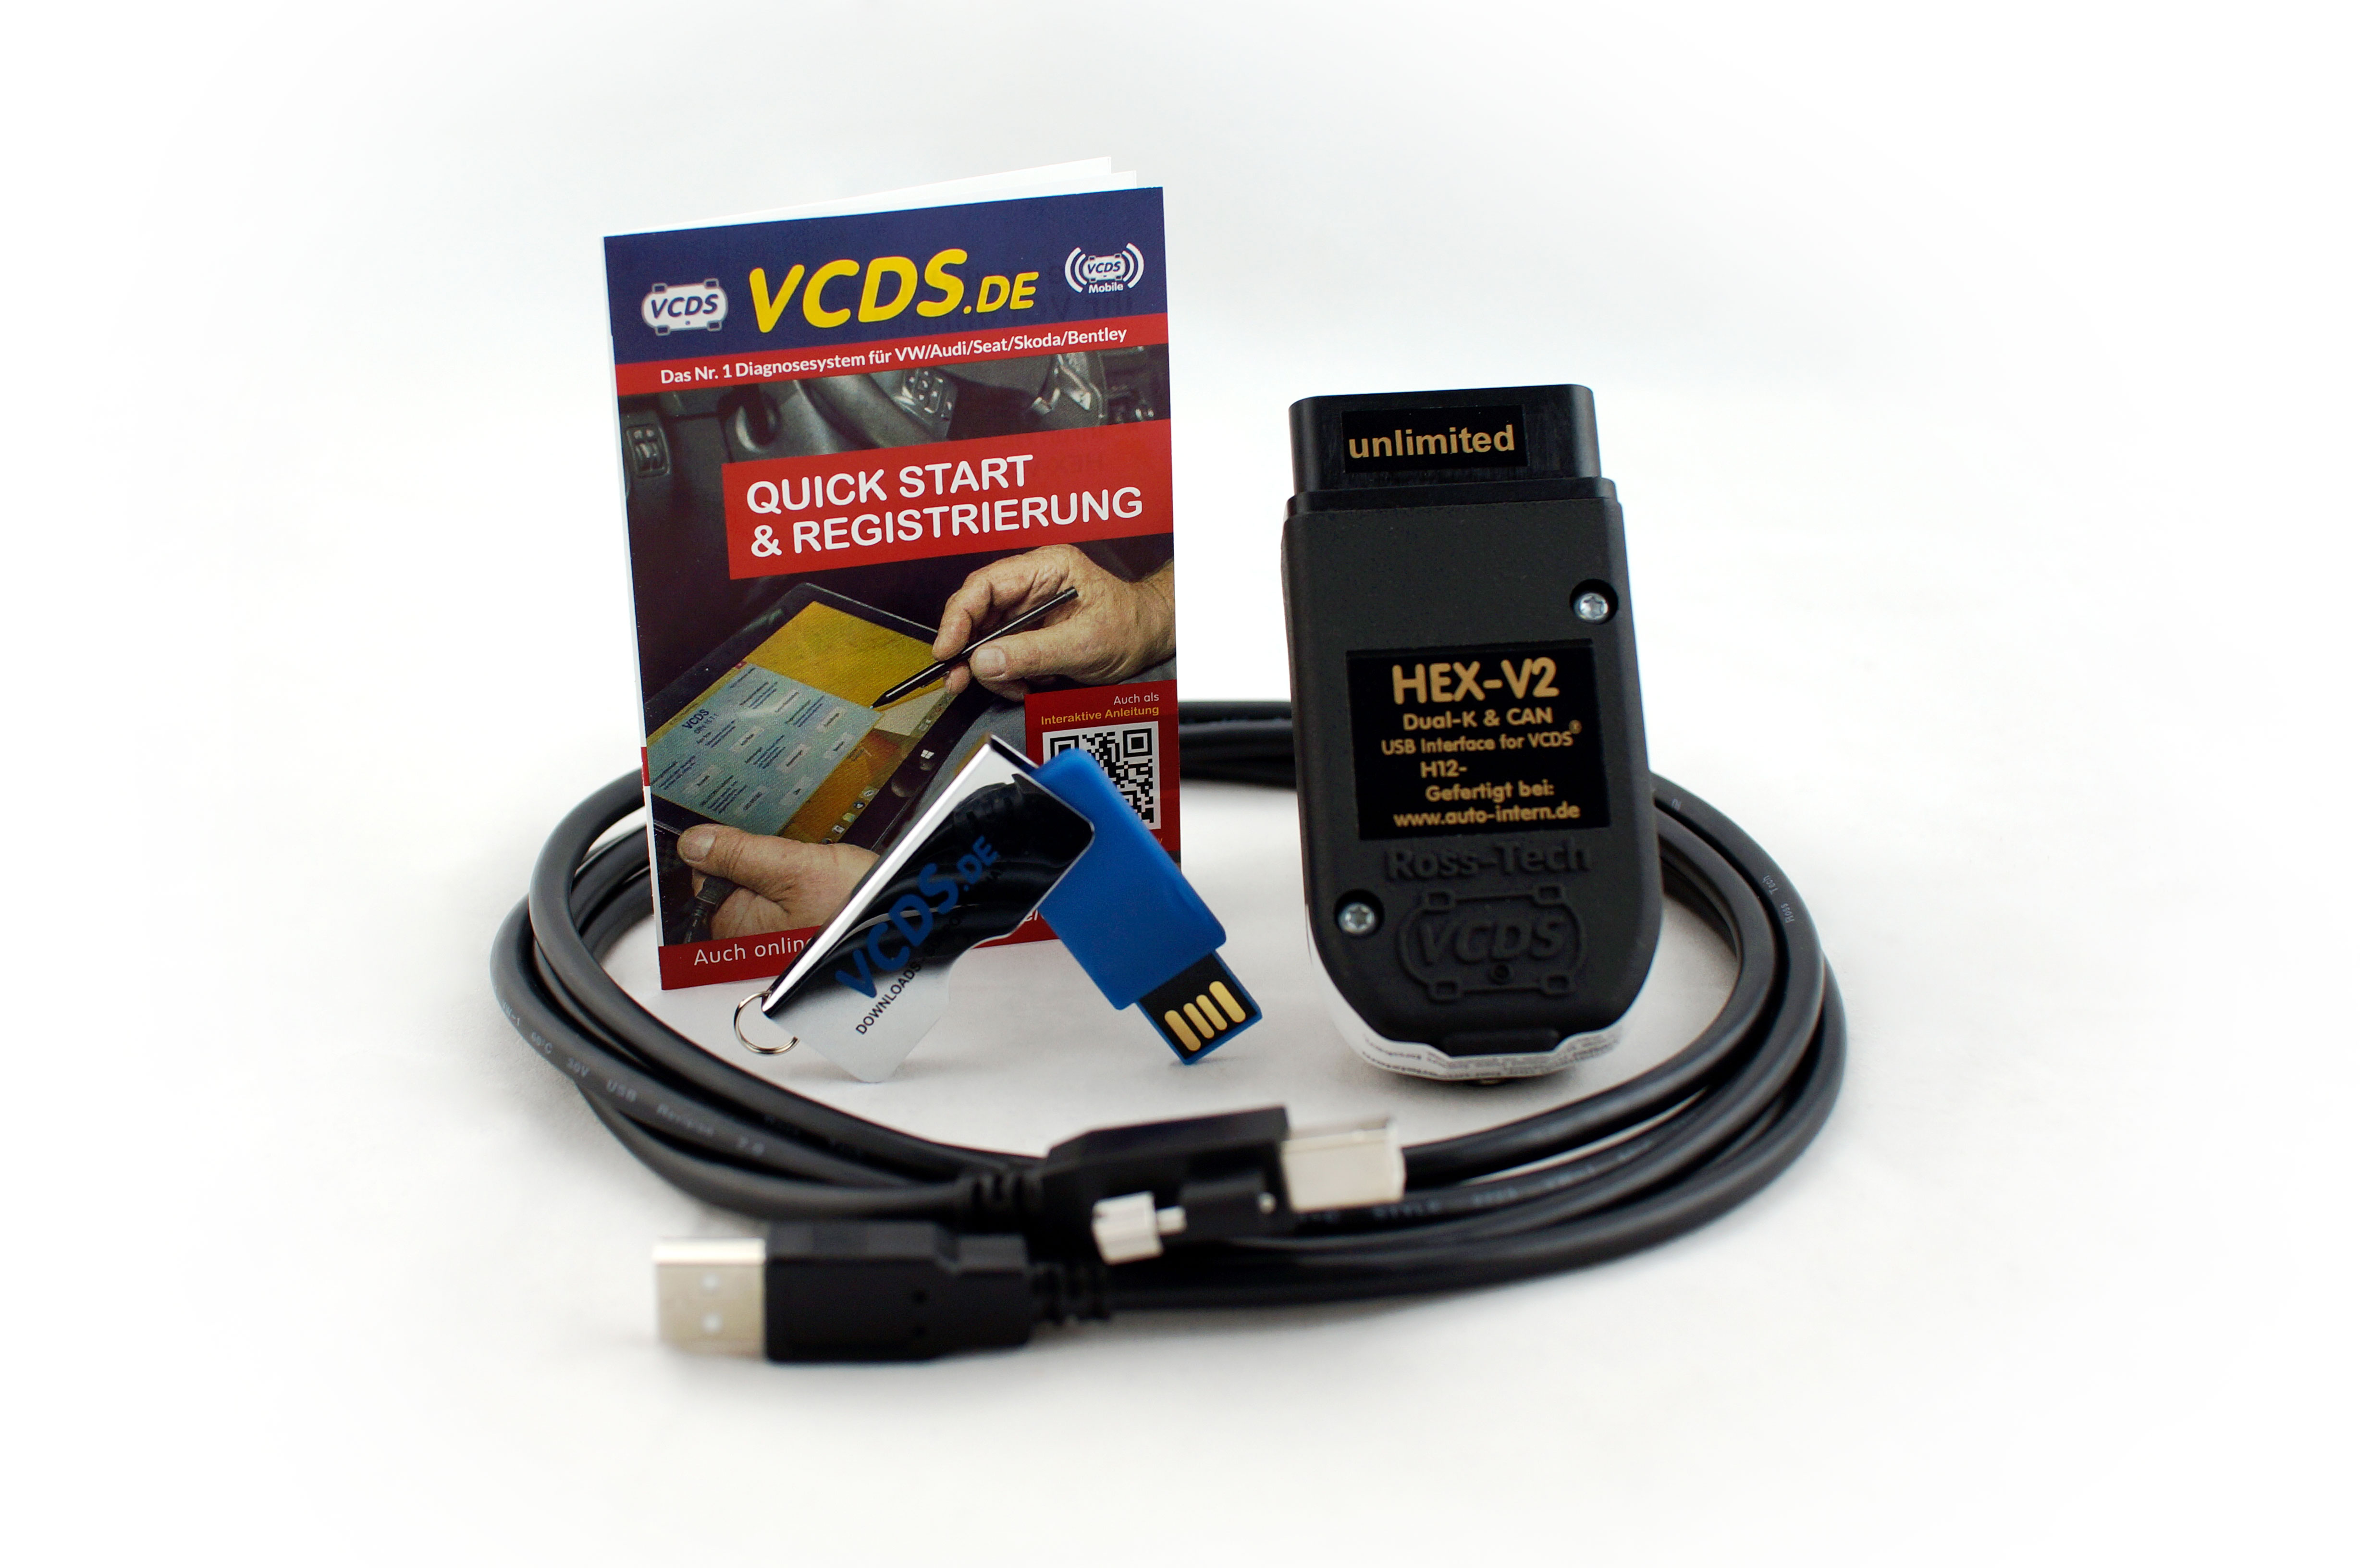
\includegraphics[width=0.8\linewidth]{obd_device}
  \caption{Picture of an OBD device}
  \label{fig:obd}
\end{figure}
Discuss the evolution from traditional On-Board Diagnostics (OBD) to advanced off-board diagnostic tools. Highlight limitations in deep signal analysis for both internal combustion and electric vehicles.

\subsection{Future Challenges in ICEV and BEV}
Outline upcoming diagnostic challenges posed by complex powertrains, high-voltage systems, and the convergence of software-defined vehicles.

\subsection{Interesting Technologies for Upcoming Car Diagnostic Systems}
\subsubsection{Oszilloscopes}
\begin{figure}[ht]
  \centering
  \includegraphics[width=0.8\linewidth]{oscilloscopes}
  \caption{Three different Oscilloscopes}
  \label{fig:scopes}
\end{figure}
Review the role of high-speed waveform capture in pinpointing transient faults.

\subsubsection{ML for Signal Clustering}
\begin{figure}[ht]
  \centering
  \includegraphics[width=0.8\linewidth]{waveforms_good_bad}
  \caption{Two waveforms: a bad and a good measurement of a compression cycle}
  \label{fig:waveforms_good_bad}
\end{figure}
Describe machine learning techniques to automatically compare live measurements against labeled “good” datasets.

\subsubsection{REST and WebSockets}
Discuss the use of HTTP REST for case management and WebSocket channels for streaming real-time data.

\subsubsection{Scope-Driver and HTTP Server}
\begin{figure}[ht]
  \centering
  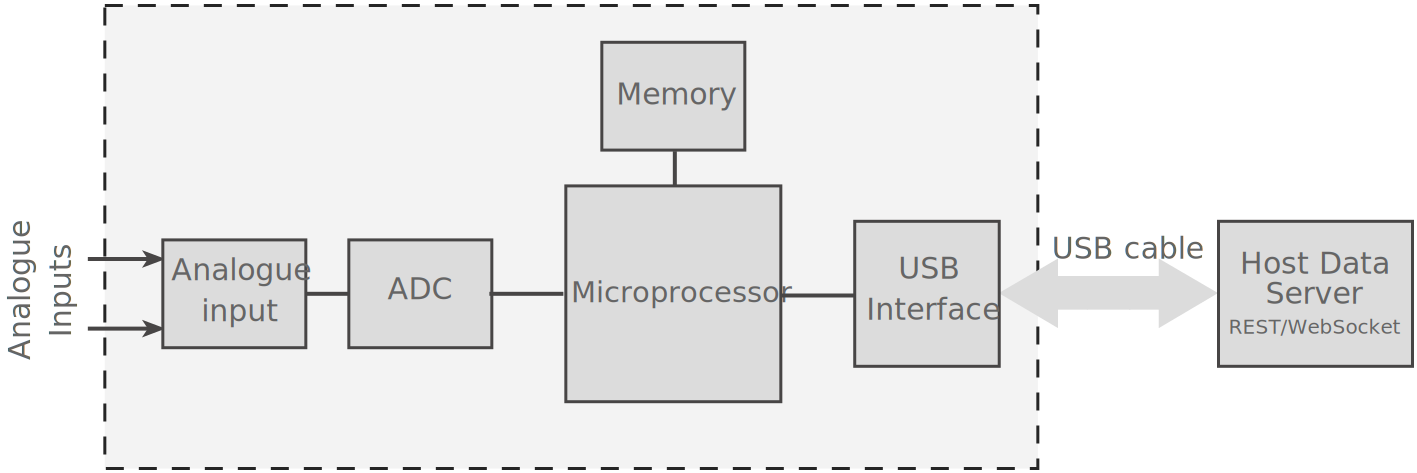
\includegraphics[width=0.8\linewidth]{data_server_architecture}
  \caption{Architecture diagram: scope connected to server via libusb and server providing REST/WebSocket}
  \label{fig:data-server}
\end{figure}
Introduce the concept of a driver plugin (shared object) coupled with an HTTP server for flexible data acquisition.

% 2. Proposed System
\section{Proposed System}
\subsection{Overview}
\begin{figure}[ht]
  \centering
  \includegraphics[width=0.8\linewidth]{system_architecture}
  \caption{Federated ecosystem architecture: data flow from scopes to AI services to technician UI}
  \label{fig:system_architecture}
\end{figure}
Provide a high-level overview of the federated ecosystem, showing secure data flows and component interactions.

\subsection{Proof-of-Concepts}
Summarize laboratory and field tests demonstrating secure data exchange and basic AI inference.

\subsection{Demonstrator}
\begin{figure}[ht]
  \centering
  \includegraphics[width=0.8\linewidth]{early_scope}
  \caption{Early-Scope measurement prototype}
  \label{fig:early-scope}
\end{figure}

\begin{figure}[ht]
  \centering
  \includegraphics[width=0.8\linewidth]{old_gui_omniview}
  \caption{Legacy GUI: OmniView}
  \label{fig:gui}
\end{figure}

\begin{figure}[ht]
  \centering
  \includegraphics[width=0.8\linewidth]{data_api}
  \caption{Data gathering API interface}
  \label{fig:data-api}
\end{figure}
Detail the integrated pilot installation in partner workshops, including hardware setup and user interface snapshots.

% 3. Results
\section{Results}
\subsection{Technical Readiness}
Report on system stability, latency, and throughput based on pilot metrics.

\subsection{Usage and Feedback}
Summarize technician survey results and adoption rates in participating workshops.

\subsection{Gathered Data}
Provide statistics on the volume, variety, and quality of collected waveform datasets.

% 4. Summary
\section{Summary}
Recap the key achievements: ecosystem architecture, live diagnostics, and workshop upskilling.

% 5. Outlook
\section{Outlook}
Discuss future work, including integration of the OmnAIScope platform, advanced federated ML modules, and expanded partner networks under GAIA-X.

\end{document}
